\documentclass[supercite]{Experimental_Report}

\title{Cuckoo-driven Way}
\school{计算机科学与技术学院}
\author{李茗畦}
\classnum{本硕博2001班}
\stunum{U202015630}
\instructor{金海}
\usepackage{zhnumber} % change section number to chinese
\renewcommand\thesection{\arabic{section}}
\renewcommand \thesubsection {\arabic{section}.\arabic{subsection}}
\usepackage{tikz}
\usetikzlibrary{mindmap,trees}
\usepackage{algorithm, multirow}
\usepackage{algpseudocode}
\usepackage{amsmath}
\usepackage{amsthm}
\usepackage{framed}
\usepackage{multirow}
\usepackage{multicol}
\usepackage{arydshln}
\usepackage{mathtools}
\usepackage{subcaption}
\usepackage{amsmath, amssymb, amsfonts}
\usepackage{tabu}
\usepackage{xltxtra} %提供了针对XeTeX的改进并且加入了XeTeX的LOGO, 自动调用xunicode宏包(提供Unicode字符宏)
\usepackage{bm}
\usepackage{longtable}
\usepackage{tikz}
\usepackage{pdfpages}
\usepackage{tikzscale}
\usepackage{pgfplots}
\usepackage{graphicx}
\usepackage{listings}
\usepackage{titlesec}
\usepackage{fontspec}
\usepackage{xcolor}      %代码着色宏包
\usepackage{CJK}         %显示中文宏包
\usepackage{pifont}
\usepackage{array}
\usepackage{booktabs}


\lstset{
    basicstyle=\ttfamily\fontseries{m},  % 将字体变细
    breaklines=true,
    lineskip=-0.5pt,
    columns=fullflexible,  % 配合keepspaces一起使用,保留空格
    %行号
    numbers=left,
    rulesepcolor=\color{red!20!green!20!blue!20},
    escapeinside=``,
    xleftmargin=2em,xrightmargin=2em, aboveskip=1em,
    %背景框
    framexleftmargin=1.5mm,
    frame=single,
    %背景色
    % backgroundcolor=\color[RGB]{245,245,244},
    %样式
    keywordstyle=\color{blue}\bfseries,
    identifierstyle=\ttfamily\color{black},
    numberstyle=\color[RGB]{0,192,192},
    commentstyle=\it\color[RGB]{96,96,96},
    stringstyle=\rmfamily\slshape\color[RGB]{128,0,0},
    %显示空格
    showstringspaces=false
}


\pgfplotsset{compat=1.16}

\newcommand{\cfig}[3]{
  \begin{figure}[htb]
    \centering
    \includegraphics[width=#2\textwidth]{images/#1.tikz}
    \caption{#3}
    \label{fig:#1}
  \end{figure}
}

\newcommand{\sfig}[3]{
  \begin{subfigure}[b]{#2\textwidth}
    \includegraphics[width=\textwidth]{images/#1.tikz}
    \caption{#3}
    \label{fig:#1}
  \end{subfigure}
}

\newcommand{\xfig}[3]{
  \begin{figure}[htb]
    \centering
    #3
    \caption{#2}
    \label{fig:#1}
  \end{figure}
}

\newcommand{\rfig}[1]{\autoref{fig:#1}}
\newcommand{\ralg}[1]{\autoref{alg:#1}}
\newcommand{\rthm}[1]{\autoref{thm:#1}}
\newcommand{\rlem}[1]{\autoref{lem:#1}}
\newcommand{\reqn}[1]{\autoref{eqn:#1}}
\newcommand{\rtbl}[1]{\autoref{tbl:#1}}

\algnewcommand\Null{\textsc{null }}
\algnewcommand\algorithmicinput{\textbf{Input:}}
\algnewcommand\Input{\item[\algorithmicinput]}
\algnewcommand\algorithmicoutput{\textbf{Output:}}
\algnewcommand\Output{\item[\algorithmicoutput]}
\algnewcommand\algorithmicbreak{\textbf{break}}
\algnewcommand\Break{\algorithmicbreak}
\algnewcommand\algorithmiccontinue{\textbf{continue}}
\algnewcommand\Continue{\algorithmiccontinue}
\algnewcommand{\LeftCom}[1]{\State $\triangleright$ #1}


\newtheorem{thm}{定理}[section]
\newtheorem{lem}{引理}[section]
\colorlet{shadecolor}{black!15}

\theoremstyle{definition}
\newtheorem{alg}{算法}[section]
\def\thmautorefname~#1\null{定理~#1~\null}
\def\lemautorefname~#1\null{引理~#1~\null}
\def\algautorefname~#1\null{算法~#1~\null}
\usepackage{xcolor}
\usepackage{listings}
\usepackage[skins]{tcolorbox}
\tcbuselibrary{breakable}
\newtcolorbox{abox}[1][]{enhanced,
	fonttitle = \heiti \large \bfseries,% 标题字体设置
	colbacktitle =black,% 标题背景颜色
	coltitle=white,% 标题字体颜色
	% halign title=center,% 标题对齐方式
	attach boxed title to top left = {yshift = -5pt},
	%	将标题以box 形式放在文本框左上角,并向下移动5pt	
	%----------正文字体--------
	fontupper = \kaishu,%正文字体设置
	%colback = white,%正文背景颜色设置
	%---------边框设置---------
	arc = 4pt,%正文边框边角弧度
	%	boxed title style={arc=0pt},%标题框边角弧度
	colframe=black,%边框颜色设置
	toprule  = 1pt,%取消上边框
	rightrule = 1pt,%取消下边框
	%---------调整字体位置------
	top = 10pt,%增大正文文本与上边框距离
	%---------设置标题为默认参数,不影响其他参数的设置
	title=#1,
	breakable
}
\newcommand{\tabincell}[2]{\begin{tabular}{@{}#1@{}}#2\end{tabular}}

%修改第三级标题
\usepackage{natbib}
\newcommand{\upcite}[1]{{\setcitestyle{square,super}\cite{#1}}}



\begin{document}

\maketitle

\tableofcontents
% \pagenumbering{arabic}

\section{并行矩阵乘法}
\subsection{任务描述}
在本实验中,将需要设计一个使用OpenMP的并行程序,用于对两个矩阵进行乘法运算。具体要求如下:
\begin{enumerate}
\item 程序接受两个矩阵作为输入,并计算它们的乘积。
\item 使用OpenMP将矩阵乘法操作并行化,以加快计算速度。
\item 将矩阵数据进行划分和分配给不同的线程以实现并行计算
\item 处理并行区域的同步,避免竞态条件和数据一致性问题。
\item 利用OpenMP的并行循环和矩阵计算指令,以进一步提高并行效率。
\end{enumerate}

\subsection{算法设计}

\subsection{实验测试}

\newpage
\section{Cuckoo hash的设计}

\subsection{基本的Cuckoo hash的设计}
Cuckoo hash是由\normalcite{pagh2004cuckoo}提出。一个基本的Cuckoo哈希表由一组哈希桶和一些哈希函数组成。哈希函数的取值一般为2个,也就是说每个对象有两个哈希桶来放置。当查询一个对象有没有在哈希表中,或者在哈希表中查询一个键对应的值,需要将该对象的键分别进行两个哈希转换,到哈希表中的两个位置查询。Cuckoo hash的查询算法的伪代码如算法\ref{alg:1}所示。

\begin{algorithm}[h]
	\caption{lookup}
    {\bf Input:}查询对象的键key
	\begin{algorithmic}[1]
        \State {$i_1$=hash(key)}
        \State {$i_2$=hash(key)}
		\If {在bucket[$i_1$]中找到key or 在bucket[$i_2$]中找到key}
            \State {命中}
        \Else
            \State {未命中}
        \EndIf
	\end{algorithmic}\label{alg:1}
\end{algorithm}

当执行插入操作时,将对象的键经过哈希函数生成两个候选位置,如果这两个候选位置中有空闲位置,那么便可将这个对象放置在空闲位置中。如果这两个位置都是空闲的,那么将该对象随机选择一个位置放置;如果这两个位置都被其他对象占据了,这是便发生了哈希冲突,为了将插入对象放入哈希桶中,将这两个位置中的某一个对象驱逐出去,将插入对象放置进去。而淘汰的对象则需要从它的其他位置寻找空闲位置,或者淘汰其他的对象,直到所有的元素都在哈希表中寻找一个位置放置。一个插入操作的示意图如\ref{fig2-1}所示。x元素经过哈希变换得到的两个候选位置为2和6,两个位置分别别b和a所占,它选择驱逐a元素,a元素的另一个候选位置为4,位置4处已经放置了c,于是a淘汰c,c被放置在它的另一个候选位置1。插入操作的伪代码如算法\ref{alg:2}。当哈希表中的容量较小时,或者选用的哈希函数性能不佳时,会产生较多的哈希冲突,一次插入过程会产生较多的驱逐,我们将这样连续的驱逐操作称作一条驱逐路径。比如在上面的例子中,驱逐路径就为x$\rightarrow$a$\rightarrow$c。在实际的应用场景中,将对象从表中取出和放置可能会导致很高的延迟,因此我们总是希望驱逐路径尽可能的小。另外,一次插入操作可能会导致哈希表中出现驱逐的无限循环。一个无限循环的例子如\ref{fig2-2}所示。一般在插入时,会通过计算驱逐次数来判断是否产生无限循环,当驱逐次数超过一个阈值,就采用更新哈希函数将哈希表重构来消除插入时的哈希冲突。

\begin{figure}[htb]
	\begin{center}
		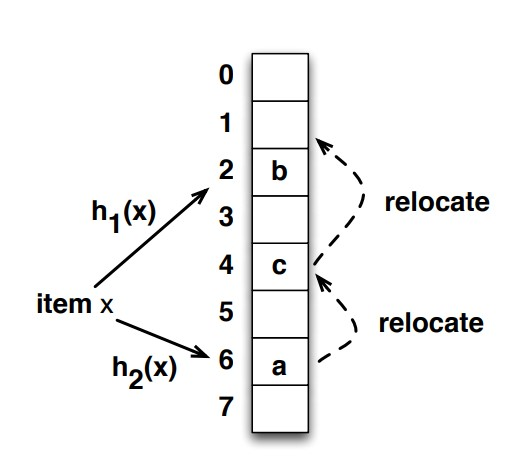
\includegraphics[scale=0.7]{./images/normol_insert.jpg}
		\caption{cuckoo的插入操作}
		\label{fig2-1}
	\end{center}
\end{figure}

\begin{algorithm}[h]
	\caption{insert}
    {\bf Input:}待放置的对象item以及键key,淘汰的最大次数$max\_kick\_cnt$
	\begin{algorithmic}[1]
        \State {$i_1$=hash(key)}
        \State {$i_2$=hash(key)}
		\If {bucket[$i_1$] or bucket[$i_2$] 是空闲的}
            \State {将item放置}
        \Else
            \State {随机选择$i_1$ or $i_2$为$kick\_item$}
            \While {淘汰次数未超过$max\_kick\_cnt$}
                \State {为$kick\_item$寻找其他位置放置}
            \EndWhile
        \EndIf
	\end{algorithmic}\label{alg:2}
\end{algorithm}


\begin{figure}[htb]
	\begin{center}
		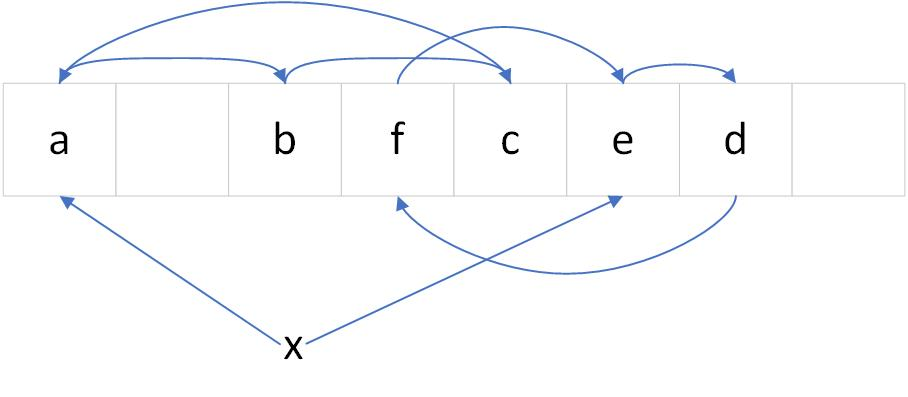
\includegraphics[scale=0.7]{./images/kick_cycle.jpg}
		\caption{驱逐的无限循环}
		\label{fig2-2}
	\end{center}
\end{figure}

\subsection{多路相联的哈希桶}
为了避免出现驱逐路径较长或者无限循环的情况,一种思路是避免哈希冲突。可以选择增加哈希表的容量、选择均匀性和抗碰撞性更强的哈希函数、增加哈希函数的数量等方法。在这里我采用了对一个哈希桶进行扩展,即在一个哈希桶中放置多个槽位,每个槽位可容纳一个元素。一个(k-b) cuckoo hash\normalcite{dietzfelbinger2005data}表示采用k个哈希函数,每个桶中有b个槽位。一般哈希函数的数量仍采用2。通过对每个哈希桶的扩展,可以大大减少发生哈希冲突的概率,避免出现较长的驱逐路径和无限循环的情况。同时可以提高哈希表的占用率。经过程序测试,一个(2-4) cuckoo hash的哈希表的占用率可超过95\%。

将哈希桶转化为多路相联后可以有效减小发生哈希冲突的概率,但是哈希表中桶的数量减少了。\normalcite{fan2014cuckoo}选择不在哈希表中存储对象的键值,而存储一个经过哈希转换得到的fingerprint,通过控制fingerprint的大小可达到压缩哈希表的目的,且可以保持相同的false positive概率。由于不在哈希表中存储原来的键值,因此在计算放置位置时,第一个位置依旧通过哈希转换由键得到,第二位置则由第一个哈希值和fingerprint经过异或得到。这样通过异或运算,在简化运算的同时,也可以通过一个位置快速获得另一个位置。


\subsection{驱逐路径的检测}
为了避免在进行驱逐时发生无限循环的情况,一种解决思路是在进行驱逐之前对哈希表进行检测,判断是不是存在一条可以采用的驱逐路径。如果不存在这样一条驱逐路径,那么在算法\ref{alg:2}的运行过程中就会出现无限循环的情况,此时花费时间在不断的驱逐过程中会造成性能的损失,应该及早选择新的哈希函数对哈希表进行重构。我们用图模型来表示哈希表,每个节点表示一个哈希桶。如果哈希表中插入一个元素x,它的两个候选位置分别为$i_1$和$i_2$,那么节点$i_1$和节点$i_2$之间便增加一条路径,表示x可以从节点$i_1$被驱逐到$i_2$或者从$i_2$驱逐到$i_1$。一条可行的驱逐路径就是从元素x要放置的节点开始,经过若干节点最终到达一个有空闲位置的节点。因此我们需要记录哈希表中还有空闲位置的节点,当选择驱逐路径时,检查从驱逐的起始节点是否有到这些空闲节点的路径。并且我们要选择路径最短的一条,因为元素的放置和取出在实际应用场景中可能会有很高的延迟,应该尽可能的少进行。然而,一个哈希表中的桶数非常大,这种方法将产生很大的内存开销。同时,在图中进行路径搜索也是一个复杂度较高的工作,在这里我们选择一个驱逐次数阈值,当插入一个元素的过程中驱逐的次数大于这个阈值时,才进行驱逐路径的检测,防止每一次插入都进行驱逐路径检测,避免对大多数插入操作造成延迟。

\newpage

\section{Cuckoo hash的实现}

\subsection{基本Cuckoo hash的实现}
Cuckoo hash选用的两个哈希函数都是Murmurhash3函数。这个哈希函数支持用户定义随机数种子,因此在生成新的哈希函数时较为方便。计算放置位置采用\normalcite{fan2014cuckoo}介绍的方法,第一个Murmurhash3函数作为用来fingerprint,第二个哈希函数用来计算放置位置。为了方便检测插入、查找等操作的正确性,我也在哈希表中放置了对象的值。其中,Murmurhash3函数的实现在静态链接库code/lib/libSMHasherSupport.a中。

哈希表table\_用一个二维数组表示,数组中的每个元素表示为一个结构Bucket,包含一个key和一个value。Cuckoo hash的具体的数据结构的定义如代码\ref{lst:data_structure}所示。其中capacity\_为哈希表的桶的数量。max\_depth\_为进行驱逐时允许驱逐的最大次数,当次数超过该阈值时则认为已经出现无限循环。kick\_cnt\_,reconstruction\_cnt\_和item\_cnt\_分别为驱逐计数,重构计数和哈希表内元素的数量。seed1\_,seed2\_,generator\_和distribution\_都是用户生成随机数的,其中seed1\_和seed2\_分别是第一个Murmurhash3和第二个Murmurhash3函数所用的随机数种子。

\begin{lstlisting}[float=h,language=C,caption={Cuckoo hash的数据结构的定义},label={lst:data_structure}]
size_t capacity_;
int max_depth_{500};
int kick_cnt_{0};
int reconstruction_cnt_{0};
size_t item_cnt_{0};
int seed1_,seed2_;
std::mt19937 generator_;
std::uniform_int_distribution<int> distribution_;
struct Bucket {
    keytype key;
    valuetype value;
};
Bucket** table_;
\end{lstlisting}

此外,Cuckoo hash主要包括以下函数:
\begin{enumerate}
\item size\_t hash1(const keytype\& key) const: 用于计算第一个哈希函数值。
\item size\_t hash2(const keytype\& key) const:和上一个函数类似,用于计算第二个哈希函数值。
\item bool kick(const keytype\& key, const valuetype\& value,id\_t kick\_pos, int depth):完成一次驱逐操作,将{key,value}从原位置中驱逐出去,选择下一个位置,如果仍然需要驱逐,则递归调用该函数。返回值为驱逐是否成功,当驱逐次数过多,将返回false表示驱逐失败。
\item bool lookup(const keytype\& key, valuetype\& value) const:完成一个查操作,根据给到的键找到对应的值,保存在value中,命中则返回true,未命中则返回false。
\item bool insert(const keytype\& key, const valuetype\& value):完成一次插入操作,成功插入则返回true,因驱逐次数过多而失败则返回false。
\item bool reconstruction():完成对哈希表的重构。该函数首先将哈希表中的元素拷贝到一个缓冲区,然后更新哈希函数,重新将缓冲区内的元素插入到哈希表中。重构成功返回true。如果仍然插入失败,将然会false,此时需要再次调用该函数直到重构成功。
\item void copy\_to\_buffer():用于将哈希表中的元素拷贝到缓冲区,并将哈希表清空。
\end{enumerate}

Cuckoo hash的实现代码在code/src/cuckoo.cpp和code/include/cuckoo.h。

\subsection{多路相联的Cuckoo hash的实现}

经过多路相联,一个哈希桶可以存放多个对象。在cuckoo hash的数据结构定义中增加一个entry\_cnt\_表示相联度,通过设置table\_的列数修改hash桶的相联度。相应的,查找、插入和驱逐等函数也应该做出修改,在一个桶中查找时应该遍历它的所有entry。同样的,在进行插入时,也可以插入到一个桶中所有的entry中。


\subsection{带有驱逐路径检测的Cuckoo hash的实现}

为了避免插入过程中的驱逐操作出现无限循环,我们在驱逐次数超过一定大小时不再继续执行可能不会停止的驱逐操作,而是检测一下哈希表中是否存在一条可行的驱逐路径。驱逐路径的起始节点是还没有放置到哈希表中的元素将要被放置到的节点,终点是一个哈希表中还存在空闲位置的节点。如果存在这么一条路径,那么在执行驱逐时便不会出现无限循环。带有循环检测的插入操作的流程图如\ref{fig3-1}所示。为了防止路径搜索影响大多数的插入操作的性能,我们只对驱逐次数达到一定大小时才执行路径检测。


\begin{figure}[htb]
	\begin{center}
		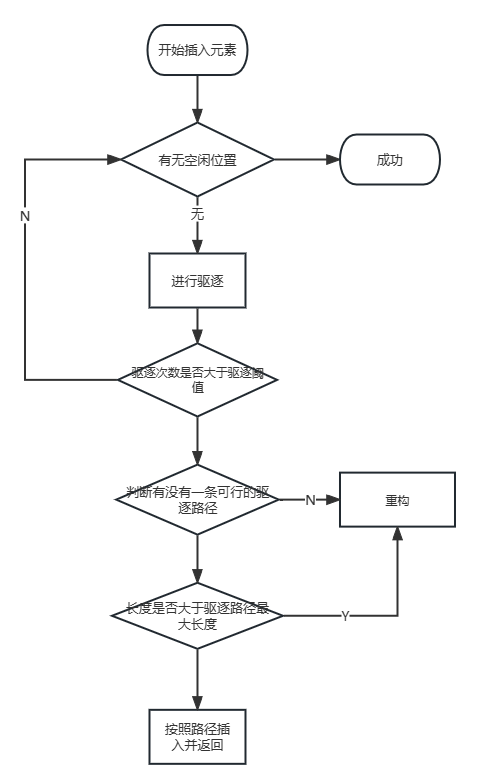
\includegraphics[scale=0.6]{./images/flow.png}
		\caption{带有驱逐检测的插入操作}
		\label{fig3-1}
	\end{center}
\end{figure}

我们将哈希表中的每一个桶看作一个节点,当在哈希表中插入一个元素x时,它有两个候选位置分别被$i_1$和$i_2$,那么节点$i_1$和$i_2$之间就存在一条路径,表示的是x可以从一个节点被驱逐到另一个节点。为了实现循环路径的检测,我们在cuckoo hash的数据结构中增加一个子类graph\_,这个子类主要包括以下成员:
\begin{enumerate}
\item id\_t max\_id\_: 表示节点的索引值的取值范围;
\item std::set<id\_t> free\_list\_:表示还有空闲位置的节点,从源节点找到一条到空闲节点的路径,就找到一条可行的驱逐路径;
\item std::unordered\_map< id\_t,std::set<id\_t> > graph\_:用邻接表表示图,图中的边表示一条驱逐路径。
\end{enumerate}

graph\_还包括以下函数:
\begin{enumerate}
\item void add\_free\_node(id\_t id):用于添加一个空闲节点;
\item void remove\_free\_node(id\_t id):用于删除空闲节点。当一个桶被占满时将调用该函数将表示该桶的节点从free\_list\_中去掉;
\item void add\_edge(id\_t id\_x,id\_t id\_y):用于图中添加一条驱逐路径。当哈希表中插入元素成功时将调用该函数;
\item bool shortest\_path\_from\_src(id\_t src\_node\_id,std::vector<id\_t>\& path) const:用于在图中寻找一条从源节点到空闲节点的驱逐路径;
\item void reconstruct():当找不到可行的驱逐路径时,用于重构图。

\end{enumerate}

其中shortest\_path\_from\_src函数基于Dijkstra算法实现,只要找到到达任何一个空闲节点的驱逐路径便可返回,将路径保存在std::vector<id\_t> path中,这样该路径一定为可到达空闲节点的路径中最近的一条驱逐路径。如果找不到这样一条驱逐路径,说明已经无法将驱逐路径上的所有点都放置到自己的候选位置上,在进行驱逐时一定会出现无限循环。这个时候需要将哈希表重构。
\newpage
\section{运行和测试}

保持哈希表的总大小不变,即哈希桶的数量和桶的相联度的乘积保持不变,依次设哈希桶的相联度为1,2,4,8,分别对这四个Cuckoo hash执行一系列插入操作,并记录插入过程中发生驱逐的次数,以及插入操作进行的的时间。

运行结果如表\ref{tab4-1}所示。可见,随着相联度的提高,哈希表的占用率也随之提高。当相联度为4时,占用率便可以超过95\%。当相联度为8的时候,哈希表的占用率几乎可以达到100\%。在测试时,我设置了一个时间阈值,当运行时间超过这个阈值时便认为当前哈希表无法插入这么大容量的数据。另外,不同相联度下的哈希表的驱逐次数阈值也是不一样的。相联度高的哈希表中,元素可选用的位置多,我就把驱逐次数阈值设定的高一些,相联度低时,元素可选用的位置少,就把驱逐次数阈值设定的高一些。这导致了运行结果中的平均驱逐次数差异较大,一些情况下重构次数较多,导致驱逐次数增加。我设定的阈值是凭借着多次测试得到的一个经验值,这可能导致我的测试结果并不十分的精确。




\begin{table}[htbp]
\caption{不同相联度下的cuckoo hash的运行结果}
\label{tab4-1}
\setlength{\tabcolsep}{6.8mm}
\begin{tabular}{cccccc}
   \toprule
     相联度& 1 & 2 & 4 & 8\\
   \midrule
占用率/\% & 51.99 & 89.79 & 97.83& 99.94	  \\
平均驱逐次数& 19.52 & 57.43 & 75.32 & 91.09  \\
每元素插入平均用时/us & 54.63 & 62.59 & 16.44 & 0.58 \\
   \bottomrule
\end{tabular}
\end{table}

\newpage

\section{总结}

通过学习和实现Cuckoo hash,自己对这个数据结构有了了解和认识,对Cuckoo hash的原理有了更深刻的理解。实现的代码文件在文件夹code中。在本课程中,我接触到了多种哈希函数,他们分别适用于不同的场景。

在这篇报告中,通过多路相联,路径检测等策略对Cuckoo hash做了一定程度的优化,提高了Cuckoo hash的空间利用率。发现提高多路检测可以提高哈希表的利用率,并通过用fingerprint代替键值\normalcite{fan2014cuckoo}来简化哈希桶位置的计算,并引入了路经检测来检查是否存在一条驱逐路径。不过,其中路径检测的优化程度比较有限,原因是Cuckoo哈希表的容量较大,对其进行依次路径搜索的时间开销很大。相比较而言,当驱逐次数超过一定阈值时直接采用暴力的重构可能是一个更有的选择。另外,受限于时间自己并没有做很严谨和详细的测试。这是我在本课程中的不足。因此,我需要一个更优的路径检测算法,并需要在本课程之外进行进一步的探索和思考。


\newpage
\bibliography{./ref.bib}
\clearpage

\end{document}
